%!TEX root = ../main.tex
\chapter{实验与分析}
在本章中,我们介绍了在两个真实的数据集上进行的实验。为了评估提出模型的评分预测效果,我们从两个方面进行实验,首先测试该模型在单个域上的预测准确性相比传统方法的提升,然后在跨域的场景下评估该模型预测的质量,并与之前单个域上的结果进行比较,说明我们提出的模型是否利用跨域的标签信息缓解了数据稀疏性问题。

\section{数据集及预处理}
在我们的实验中使用了两个免费的真实数据集:包含 $200$ 万个评分的 MovieLens\footnote{MovieLens dataset: https://grouplens.org/datasets/movielens/20m/}  数据集,以及包含 70 万个评分的 LibraryThings\footnote{LibraryThing dataset: http://www.librarything.com/}数据集,这两个数据集的评分都在 1 到 5 范围内,步长为 0.5。MovieLens 包含 72,000 个用户对 10,000 个电影标注的 100,000 个标签,LibraryThings 包含 7,000 个用户对 37,000 个书籍标注的 200 万个标签。


MovieLens 数据集中的很多评分都没有关联的标签,在没有标签的情况下,我们的模型与传统的矩阵分解方法没有区别。既然我们的目的是通过实验验证引入标签信息是否对预测评分有好处,因此我们只考虑那些至少包含一个标签的评分。为了在跨域情况下减少不必要的干扰,我们使两个数据集的评分数相同,各自截取它们的前 1,0000 个具有标签的评分。在这两个评分的子集中,数据稀疏性都超过了 $99.5\%$ , MovieLens 中的标签覆盖了 LibraryThings 中 $25.31\%$ 的标签,而 LibraryThings 中的标签覆盖了 MovieLens 中 $15.09\%$ 的标签。LibraryThings 中不同的标签数更少,但是总共的标签数却更多,我们推测这些差异可以用于解释辅助域对于目标域的评分预测影响的大小。表\ref{dataset_feature}是数据集的详细统计信息。

\begin{table}[htbp]
\centering
\caption{MovieLens 和 LibraryThings 数据集的统计信息。}
\label{dataset_feature}
\begin{tabular}{|l|c|c|}
\hline
\rowcolor[HTML]{EFEFEF} 
           & MovieLens & LibraryThing \\ \hline
评分总数       & 10000     & 10000        \\ \hline
用户数        & 540       & 530          \\ \hline
物品数        & 3944      & 6092         \\ \hline
标签数        & 7284      & 4343         \\ \hline
全部标签       & 33875     & 44259        \\ \hline
每个用户的平均评分数 & 18.52     & 18.87        \\ \hline
每个评分的平均标签数 & 3.39      & 4.43         \\ \hline
标签覆盖率      & 15.09\%   & 25.31\%      \\ \hline
数据稀疏度      & 99.53\%   & 99.69\%      \\ \hline
\end{tabular}
\end{table}

\section{实验设计}
我们设计两组实验:第一组实验测试提出的模型在单个域上的预测准确性,并与其他模型进行比较分析;另一组实验在跨域的场景下进行,对比跨域模型和之前单个域上模型的效果。
\subsection{数据集划分}
为了保证实验结果的准确性,我们采用交叉验证过程。首先将数据集的评分数据均分成五个部分,我们使用其中的一份数据作为测试集,而剩余的部分作为训练集。将这个过程重复五次,使得我们可以利用五个不同的测试集来测试模型的效果。

为了验证模型在不同数据稀疏程度下的表现,我们将选中的训练集再均分为十份,因此,为了验证在数据非常稀疏的情况下模型的表现,我们使用 $10\%$的训练数据进行实验,之后每次加入一份数据,以模拟实际系统中数据不断丰富的情况。

在跨域的场景下,目标域数据集的划分方式与上面所述相同,对于辅助域则将全部的数据划分为训练集。

\subsection{评价标准}
准确度是度量一个推荐系统预测能力的指标,通常将预测的行为与测试集上行为的重合度作为预测准确度。推荐的任务可以分为 TopN 推荐和评分预测两种:网站提供推荐服务时一般会给用户一个猜你喜欢列表,这种推荐叫做 TopN 推荐,TopN 推荐的准确度一般利用召回率(Recall)和精确率(Precision)来度量;而有些网站具有用户给物品打分的功能,评分预测就是预测用户给他未评分的物品的评分,通常用平均绝对误差(MAE)和均方根误差(RMSE)来评估预测准确度。本文使用的数据集是五分制的评分形式,因此我们的实验属于评分预测的范畴。

对于测试集中的一个用户 $u$ 和物品 $i$ ,另 $r_{ui}$ 是用户 $u$ 对物品  $i$  的实际评分,而 $\hat{r_{ui}}$  是推荐算法给出的预测评分,那么 MAE 定义为:
\begin{equation}
MAE = \dfrac   {\sum\limits_{u,i \in T}  |r_{u,i} - \hat{r_{ui}}| } {|T|}.
\end{equation}
RMSE 采用均方根的形式计算预测误差,它的定义为:
\begin{equation}
RMSE = \sqrt{  \dfrac   {\sum\limits_{u,i \in T}  (r_{u,i} - \hat{r_{ui}}) ^2 } {|T|}   }.
\end{equation}
相比于 MAE,RMSE 的评价标准更加严格,它在防止过拟合方面更加灵敏,所以我们在进行模型参数训练时采用 RMSE 来衡量模型推荐效果。

我们将提出的模型与两个之前提到的 SVD 和 UserItemTags 模型进行对比,其中 SVD 模型无法利用辅助域的额外信息,因为两个域的用户和物品是没有交集的。在进行不同模型的对照实验时,为了全面地评估模型的性能,我们也比较了不同模型的 MAE 的大小。

\subsection{参数设置}
我们通过实验分析不同参数组合对模型的影响,在实验数据集上将模型调整到最优状态。

$f$ 作为潜在特征向量维度,对模型的推荐效果和运算效率至关重要,当 $f$ 值比较小时,时间复杂度会比较低,但是可能会损失预测的准确度,因此我们需要在两者之间找到一个折中的 $f$ 值。首先根据经验固定其他参数,对不同的 $f$ 取值进行实验,确定之后实验中 $f$ 的值。
\begin{figure}[htbp]
\centering
\subfigure[MovieLens]{
\label{fig:nfactors:movielens}
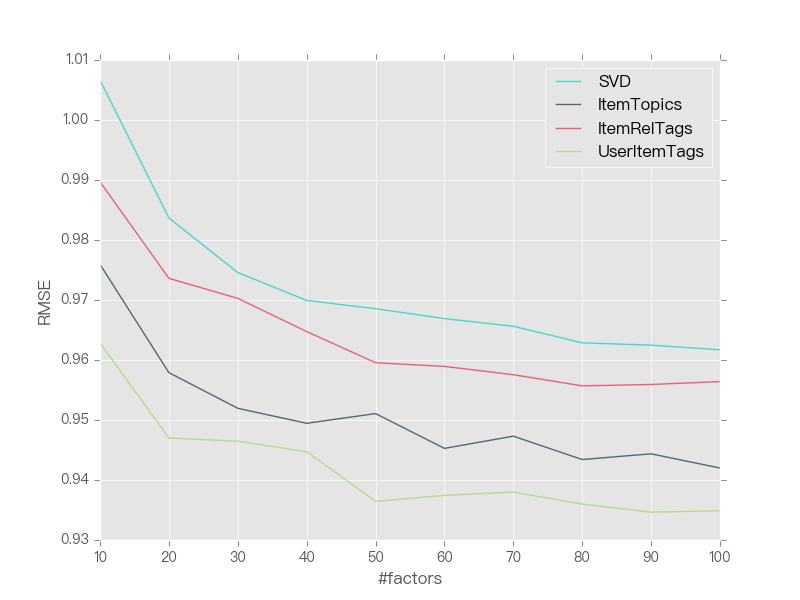
\includegraphics[width=0.48\linewidth]{images/factors1.png}
}
\subfigure[LibraryThings]{
\label{fig:nfactors:librarythings}
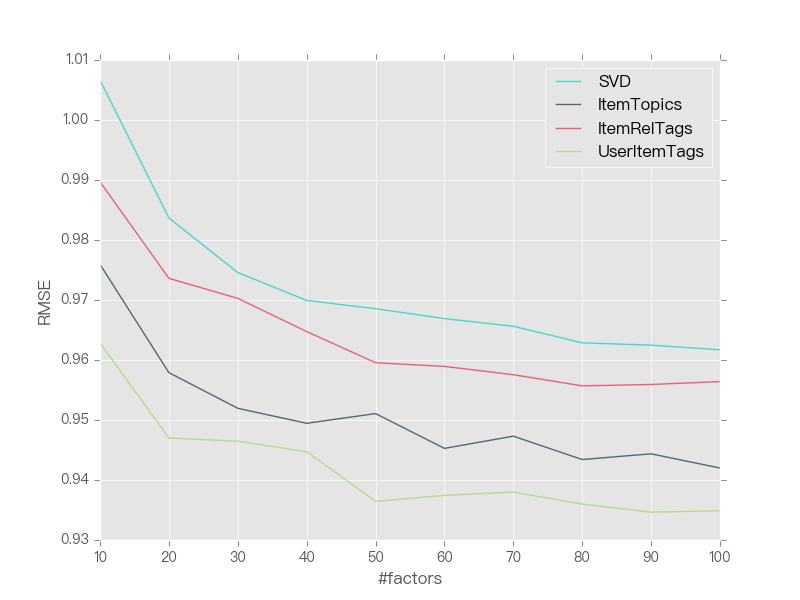
\includegraphics[width=0.48\linewidth]{images/factors1.png}
}
\caption{特征向量维度 $f$ 对模型 RMSE 的影响。}
\label{fig:nfactors}
\end{figure}
图 \ref{fig:nfactors} 显示了 $f$ 在 10-100 之间取值时不同模型的预测效果,可以看到随着 $f$ 的增大,各模型的准确度呈上升的趋势,并逐渐趋于稳定。处于对计算复杂性的考虑,我们在之后实验中将 $f$ 设置为 100。

固定参数 $f$ 之后,我们利用网格搜索的方式获得其它参数的最优值,各模型在两个数据集上的最优参数见表 \ref{params}。

\begin{table}[htbp]
\centering
\caption{模型的最优参数。}
\label{params}
\begin{tabular}{|l|c|c|c|c|}
\hline
             & \multicolumn{2}{c|}{MovieLens} & \multicolumn{2}{c|}{LibraryThings} \\ \hline
             & $\gamma$      & $\lambda$      & $\gamma$        & $\lambda$        \\ \hline
SVD          & 0.01          & 0.04           & 0.01            & 0.02             \\ \hline
UserItemTags & 0.01          & 0.04           & 0.01            & 0.01             \\ \hline
ITCF         & 0.01          & 0.02           & 0.01            & 0.02             \\ \hline
TTCF         & 0.005         & 0.002          & 0.04            & 0.01             \\ \hline
\end{tabular}
\end{table}

\subsection{LDA 主题建模}
本文采用开源的 Python 程序包 lda\footnote{http://pythonhosted.org/lda/} 进行标签主题建模,它以吉布斯采样的方式实现了隐式狄利克雷分布(LDA)。我们在实验中设置 lda 的参数 $\alpha=0.1​$ 、$\eta = 0.01​$ ,迭代次数为 2000。为了观察提取主题的有效性,我们设置主题数 $K=20$ ,表\ref{Topics}是通过训练 LDA 模型得到的两个数据集上的 Top 词表。

我们发现属于相同主题的标签项具有相近的意思,即利用主题建模完成了标签聚类。因此,根据每个主题对应的词表可以很容易解释主题的含义,我们将凭经验总结的主题词列在了每个主题的上面。

\begin{table}[htbp]
\footnotesize
\centering
\caption{从两个数据集学习到的主题。}
\label{Topics}
\begin{tabular}[c]{ccccccc}
\hline
\hline
\multicolumn{7}{c}{MovieLens 的主题}                                                             \\
喜剧        & 间谍         & 冒险           & 黑色幽默        & 犯罪       & 科幻        & 战争           \\ \hline
comedy    & politics   & fantasy      & dark comedy & quentin  & sci-fi    & true story   \\ 
funny     & espionage  & adventure    & quirky      & violence & dystopia  & world war ii \\ 
animation & religion   & johnny depp  & satire      & action   & aliens    & classic      \\ 
pixar     & action     & magic        & drugs       & crime    & space     & war          \\ 
disney    & tom cruise & stylized     & cult        & revenge  & robots    & history      \\ 
parody    & thriller   & martial arts & witty       & drugs    & future    & tom hanks    \\ 
christmas & conspiracy & surreal      & satirical   & violent  & adventure & racism       \\ 
hilarious & corruption & fairy tale   & zombies     & mafia    & cyberpunk & prison       \\ \hline
% \noalign{\bigskip}  
\hline
\hline
\multicolumn{7}{c}{LibraryThings 的主题}                                                             \\ 
魔幻        & 历史         & 幽默           & 经典        & 传记       & 科幻        & 惊悚           \\ \hline
fantasy    & history   & humor      & classic & nonfiction  & sci-fi    & mystery   \\ 
magic     & religion  & humour    & literature      & memoir & novel  & crime \\ 
discworld & philosophy   & comics  & poetry      & history   & dystopia    & thriller      \\ 
mythology     & war     & satire        & manga       & biography    & space     & suspense          \\ 
wizards    & christianity & comedy     & british        & reference  & aliens    & murder      \\ 
novel    & nonfiction   & funny & drama       & travel    & fantasy    & detective    \\ 
dragons & biography & surreal      & romance   & autobiography  & time travel & adventure       \\ 
adventure & politics & art   & england     & essays    & fiction & novel       \\ \hline
\hline
\end{tabular}
\end{table}

\section{实验结果分析}
本节中,我们按照实验设计中的方法得到模型的参数,并对模型进行训练。通过对比不同模型间的推荐准确性 RMSE,分析各模型的优劣。第一组实验测试在单个域上的预测准确性,第二组是在跨域的场景下实验,并将得到的结果与之前单个域进行对比。

\subsection{单个域推荐}
为了验证本文提出的两个模型的预测效果,我们将它们与两个优秀的推荐算法进行比较:SVD 模型,即基于矩阵分解的协同过滤算法;UserItemTags 模型,在 SVD 中结合了目标用户对目标物品的标签信息。我们从 RMSE 和 MAE 两个角度分别在 MovieLens 和 LibraryThings 数据集上衡量各模型的性能,并将实验结果数据用柱状图展示出来,如图 \ref{fig:bar} 所示,其中数值越低表示模型的推荐准确度越高。
\begin{figure}[!htbp]
\centering
\subfigure[RMSE]{
\label{fig:bar:rmse}
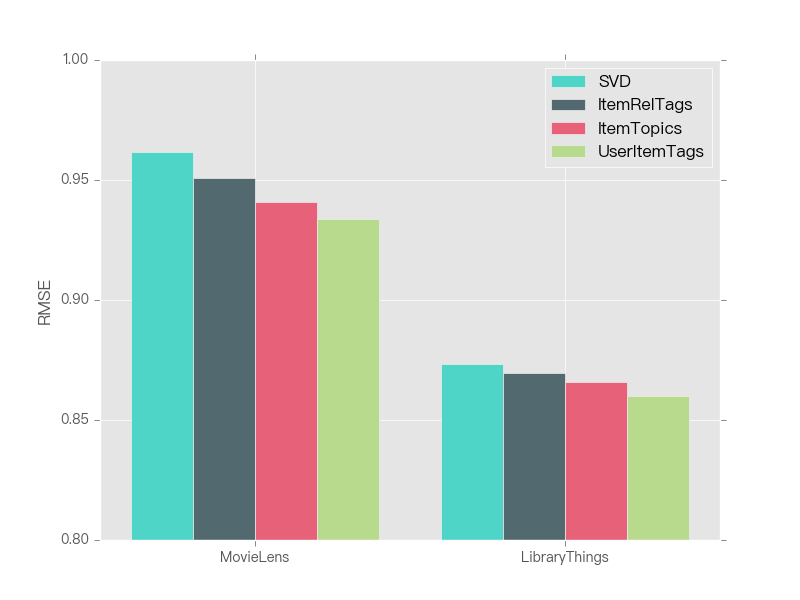
\includegraphics[width=0.48\linewidth]{images/bar_rmse.png}
}
\subfigure[MAE]{
\label{fig:bar:mae}
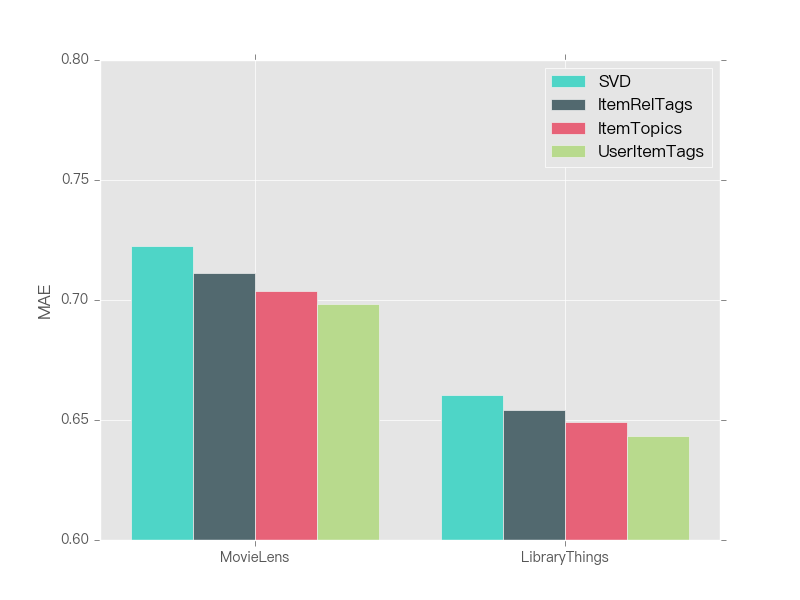
\includegraphics[width=0.48\linewidth]{images/bar_mae.png}
}
\caption{不同模型的推荐准确度对比。}
\label{fig:bar}
\end{figure}

从结果中看出,我们提出的两个模型 ITCF 和 TTCF 在预测准确性上都优于传统的 SVD 矩阵分解算法,由此证明了引入额外的标签信息对于预测效果的提升是有帮助的。因为 UserItemTags 模型必需目标用户对目标物品的标签,因此在推荐准确性上强于我们的模型,但是我们的模型解除了这项限制,具有更广泛的适用性。对于我们提出的两个模型,它们都利用了物品的标签信息,相比于 ITCF 模型,TTCF 利用主题建模对标签进行了聚类,去除了冗余信息的同时扩充了标签的含义,使得模型的推荐效果有了显著提升。
\begin{figure}[!htbp]
\centering
\subfigure[MovieLens]{
\label{fig:single_plot:MovieLens}
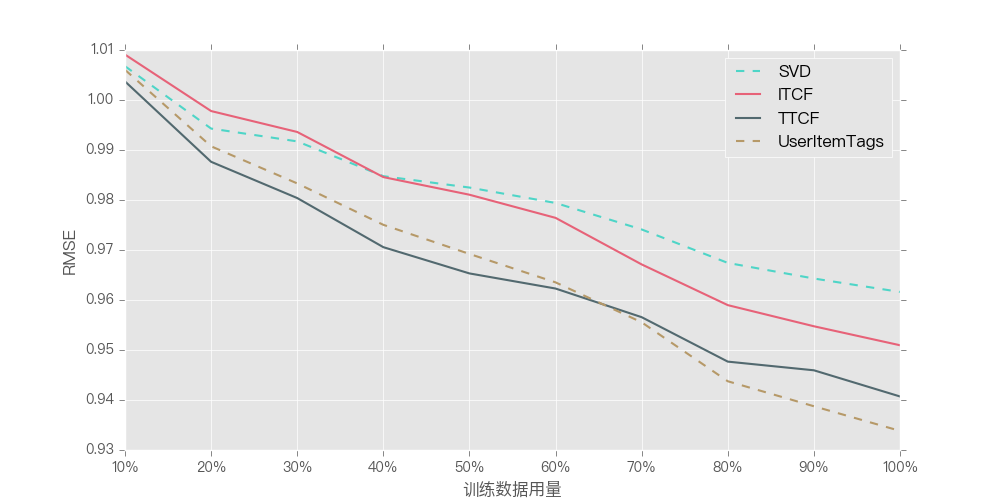
\includegraphics[width=\linewidth]{images/plot1.png}
}
\subfigure[LibraryThings]{
\label{fig:single_plot:LibraryThings}
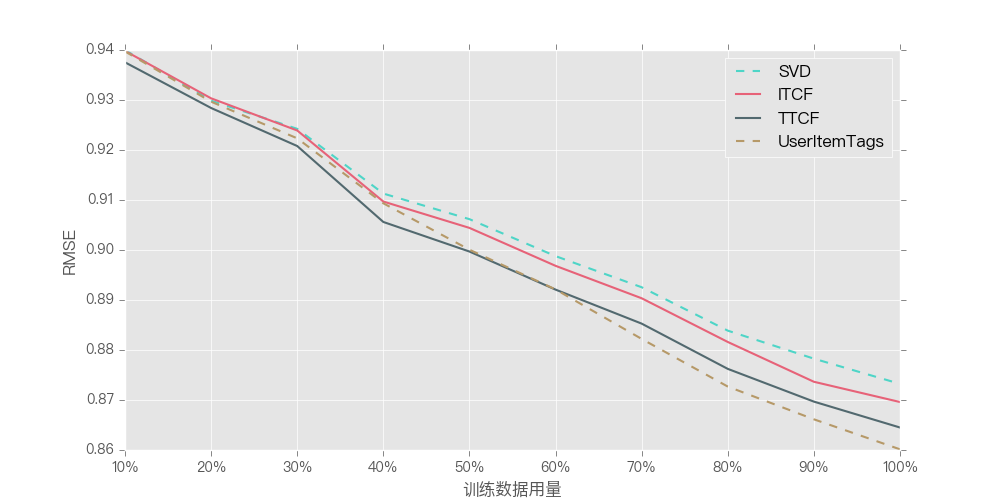
\includegraphics[width=\linewidth]{images/plot2.png}
}
\caption{不同数据用量下模型的 RMSE 对比。}
\label{fig:single_plot}
\end{figure}

接下来我们得到了在不同数据稀疏程度下各个模型的实验结果,图 \ref{fig:single_plot} 展示了不同模型的 RMSE 在各个数据用量上的数值.可以看出,在数据用量比较多的情况下,模型的预测准确度与上面得到的结果相同,但是在数据比较稀疏时,各模型表现出的性能有些不同。由于 TTCF 模型利用聚类扩充了标签含义,使得它仅利用少量标签即可获得很好的预测效果,因此在数据用量比较小时该模型的准确性超过了 UserItemTags 模型的准确性,可以说 TTCF 模型很好地缓解了数据稀疏性问题。另外,我们看到在 MovieLens 数据集上,当数据用量小于 $40\%$ 的情况下,ITCF 模型的预测准确性甚至低于 SVD 模型,我们推测这是因为当物品的标签很少时,少量的标签不能准确地描述物品的性质,甚至对评分预测产生了误导,而随着可利用的物品标签的丰富,预测准确性也逐渐超过了 SVD 模型。


\subsection{跨域推荐}
接下来我们在两个跨域的场景下验证提出的 Cross-TTCF 模型,第一种情况将 MovieLens 作为目标域,LibraryThings 作为辅助域,第二种情况将 LibraryThings 作为目标域,而 MovieLens 作为辅助域。同样,为了验证不同数据稀疏程度下模型的性能,我们使用不同的数据用量进行实验,并将得到的结果与单个域的模型进行对比。

图 \ref{fig:cross_plot}展示了不同数据用量下模型的预测准确度,可以看出,相比于只使用单个域的数据,跨域模型利用辅助域的评分和标签信息从整体上提升了目标域的推荐性能。
然而,在 LibraryThings 作为目标域的情况下,我们看到当数据用量很少时(少于 20\%),辅助域的标签信息并不能帮助提升预测的准确性。我们认为这是因为辅助域(MovieLens)中的标签覆盖了相对更多的目标域(LibraryThings)中的标签,因此当目标域只使用 10\% 的数据时,辅助域中标签和评分的关系会对预测模型造成很大的影响。换句话说,模型利用标签预测了辅助域中的评分,而不是目标域的评分。
\begin{figure}[!h]
\centering
\subfigure[MovieLens 作为目标域,LibraryThings 作为辅助域]{
\label{fig:cross_plot:MovieLens}
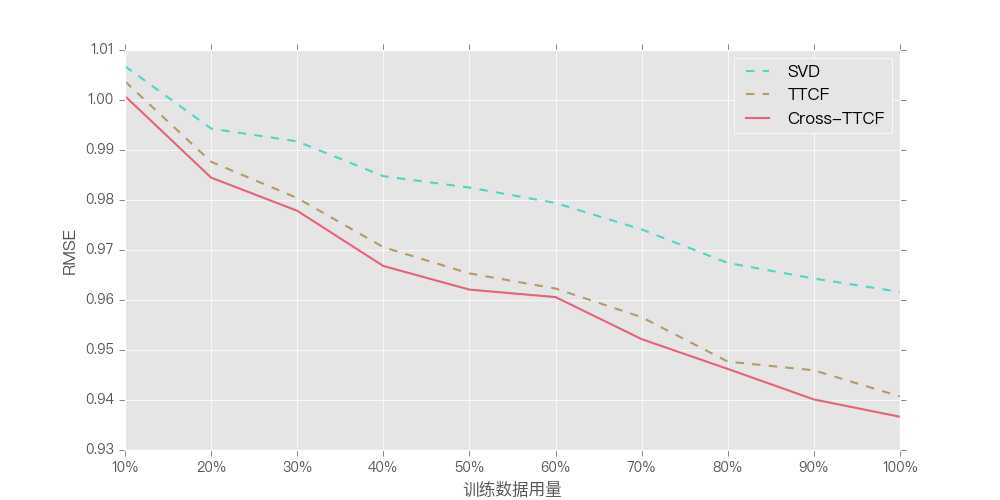
\includegraphics[width=\linewidth]{images/cross1.png}
}
\subfigure[LibraryThings 作为目标域,MovieLens 作为辅助域]{
\label{fig:cross_plot:LibraryThings}
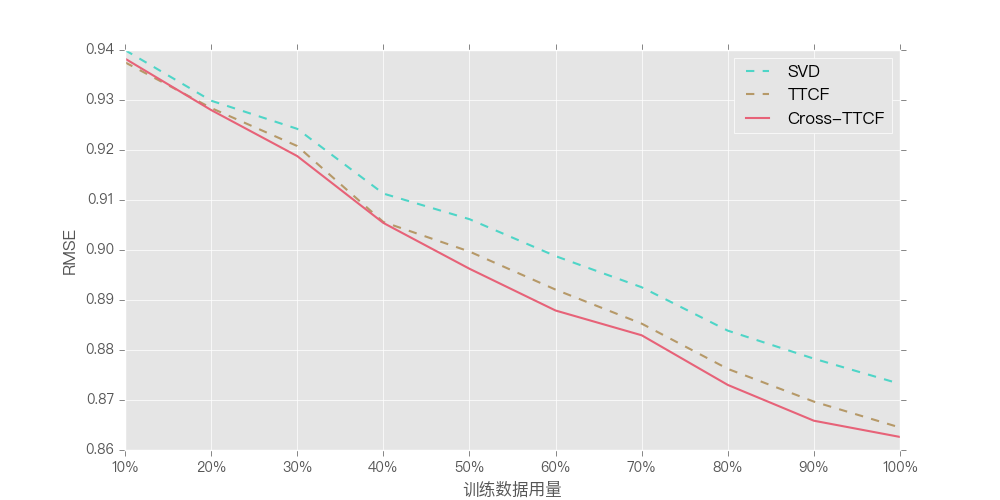
\includegraphics[width=\linewidth]{images/cross2.png}
}
\caption{单个域和跨域模型的 RMSE 对比。}
\label{fig:cross_plot}
\end{figure}

\section{本章小结}
本章中,我们首先对实验数据集进行了预处理,并得到了数据集的统计信息。之后我们阐述了实验的设计方案,采用 5 折交叉验证评估模型的预测准确性,利用网格搜索获取模型的最优参数,并解释了标签主题的意义。我们从两个方面进行对比实验并得出结论:在单个域上,我们提出的 TTCF 模型相比于传统矩阵分解模型具有明显优势,并且在数据比较稀疏的情况下,TTCF 模型的预测性能超过了 UserItemTags 模型,说明结合标签主题的模型对于缓解数据稀疏性问题具有良好的效果;在跨域的场景下,通过与单个域模型的对比,证明了我们的模型利用辅助域的标签和评分信息提升了目标域的推荐准确性,并讨论了跨域推荐中存在的问题。


